\section{Cohomology and Control: Kepler’s Laws Reimagined}

\subsection{The Language of Holes: Eilenberg, Steenrod, and the Birth of Cohomology}

In the mid-20th century, a pair of mathematicians—\textbf{Samuel Eilenberg} and \textbf{Norman Steenrod}—set out to unify the rapidly growing jungle of tools used to study the shape and structure of spaces. What emerged was a powerful abstraction: \textbf{cohomology theory}, a general framework for detecting and classifying the \textit{holes} in a space.

But what do we mean by “holes”?

Let’s build some intuition.

\subsection{What Counts as a Hole?}

- Take a straight line with a point removed. If you place two points on either side of the missing point, there's no continuous way to slide one into the other—something is blocking the path. That "gap" is a \textbf{0-dimensional hole}.

- Now consider a plane with a point missing. Any two points can be connected by a path that avoids the missing spot, but if you wrap a rubber band around the hole, you can’t shrink it to a point without crossing the void. That’s a \textbf{1-dimensional hole}.

- In 3D space, removing a point means loops can still shrink—just dodge the missing point. But if you surround the point with a sphere, that surface can't collapse without slipping into the hole. That’s a \textbf{2-dimensional hole}.

- Or imagine a torus—the surface of a donut. There are two fundamental 1-dimensional loops you can't shrink: one through the hole, one around the body. These loops represent \textit{independent generators} of 1-dimensional holes.

What makes something a hole in this context?

\begin{itemize}
    \item It has \textbf{no boundary}.
    \item It is \textbf{not the boundary of something else}.
\end{itemize}

This seemingly simple idea is at the heart of \textbf{homology} and \textbf{cohomology}. And what Eilenberg and Steenrod realized was this: rather than studying holes through ad hoc geometric or analytic tricks, we could define a cohomology theory axiomatically. Their axioms became the blueprint for modern algebraic topology—guaranteeing that any "reasonable" way of counting holes would satisfy properties like homotopy invariance, exactness, and excision.

\subsection{From Simplices to Forms: de Rham Cohomology}

One particularly elegant instance of cohomology comes from calculus and physics: \textbf{de Rham cohomology}.

Here’s the idea.

In differential geometry, we study \textbf{differential forms}—expressions made from functions and “infinitesimal directions” like \( dx, dy, dz \):

\begin{itemize}
    \item \textbf{0-forms} are just functions \( f(x, y, z) \)
    \item \textbf{1-forms} look like \( f\,dx + g\,dy + h\,dz \)
    \item \textbf{2-forms} look like \( f\,dx \wedge dy + g\,dx \wedge dz + h\,dy \wedge dz \)
    \item And so on.
\end{itemize}

These forms can be differentiated:  
Differentiating a \( k \)-form yields a \( (k+1) \)-form. And there’s a key rule: the derivative of a derivative is always zero: \( d^2 = 0 \). This structure is called a \textbf{cochain complex}—and it’s the raw material for defining cohomology.

We say:
\begin{itemize}
    \item A form is \textbf{closed} if \( d\omega = 0 \)
    \item A form is \textbf{exact} if \( \omega = d\eta \) for some \(\eta\)
\end{itemize}

This mirrors our geometric intuition:
\begin{itemize}
    \item “Closed” = has no boundary
    \item “Exact” = is the boundary of something
\end{itemize}

A form is a cohomological “hole” if it is closed but not exact. The space of all such holes is the \textbf{de Rham cohomology group}:

\[
H^k_{\text{dR}}(M) = \frac{\text{Closed } k\text{-forms}}{\text{Exact } k\text{-forms}}
\]

This means two things:

\begin{itemize}
    \item De Rham cohomology gives an analytic method to detect topological features—holes, voids, obstructions.
    \item For smooth manifolds, de Rham cohomology turns out to be \textit{isomorphic} to singular and simplicial cohomology.
\end{itemize}

That’s the magic. Whether you count holes by deforming triangles, integrating forms, or solving equations, the answer is the same. This universality is exactly what Eilenberg and Steenrod’s axioms predict—and why cohomology is more than a formula. It's a \textbf{language} shared across geometry, topology, and physics.

\begin{tcolorbox}[colback=blue!5!white, colframe=blue!75!black, title={Historical Sidebar: The Axioms of Eilenberg–Steenrod}]
In the 1940s, Eilenberg and Steenrod formalized the concept of a cohomology theory with five core axioms: homotopy, exactness, excision, dimension, and additivity. Any functor from topological spaces to abelian groups that satisfies these axioms can be considered a legitimate cohomology theory. Their framework allowed a comparison between wildly different approaches—simplicial, singular, Čech, de Rham—and proved that for “nice” spaces, they all say the same thing.
\end{tcolorbox}

\subsection{A Physical Example}

Take the 1-form:

\[
\omega = \frac{-y}{x^2 + y^2}\,dx + \frac{x}{x^2 + y^2}\,dy
\]

This form is closed—but not exact on the plane with the origin removed. It detects the 1-dimensional hole in that punctured plane. If you’ve studied complex analysis, you’ll recognize it as the real version of \( \frac{dz}{z} \), and it’s exactly why a path integral around the origin yields \( 2\pi i \)—a residue that survives because of the hole.

That’s not just clever calculus—it’s de Rham cohomology in action.


\subsection{From Areas to 2-Forms: The Hidden Geometry of Orbits}

We’ve seen how Eilenberg and Steenrod formalized cohomology as a universal language for counting holes—linking geometry, algebra, and analysis. We’ve seen how de Rham cohomology detects global topological features through the behavior of differential forms.

But cohomology doesn’t just live in abstract shapes or punctured planes.

It governs the motion of the planets.

Kepler’s Second Law—\textit{equal areas in equal times}—is often framed in terms of angular momentum or conservation laws. In Newtonian mechanics, it reflects the absence of torque. In control theory, it corresponds to a conserved costate under rotational symmetry.

But cohomologically, it reflects something deeper.

The “swept area” isn’t just a geometric fact—it’s the integral of a closed 2-form over a moving cycle. Let \( \omega \) be that 2-form. Then:

\[
d\omega = 0
\]

This means \( \omega \) defines a de Rham cohomology class—one that remains invariant as the planet traces its orbit. In cohomological terms:

\begin{quote}
\textbf{Kepler’s law encodes the preservation of a global 2-form class, not just a local quantity.}
\end{quote}

This moves us from the realm of forces and accelerations to a global language of conservation—one that lives in the cohomology of phase space.

\subsection{The Pontryagin Hamiltonian and Cohomological Invariants}

In optimal control theory, the Pontryagin Hamiltonian

\[
\mathcal{H}(q, p, u) = p \cdot f(q, u) + L(q, u)
\]

generates the system’s dynamics. Here, \( q \) represents the system’s state, \( p \) is the costate (dual variable), \( u \) is the control, and \( L \) is the running cost.

The resulting flow preserves the symplectic form:

\[
\omega = dp_i \wedge dq^i
\]

This symplectic 2-form is closed—\( d\omega = 0 \)—and thus defines a nontrivial element in de Rham cohomology. Even when the system is under control (i.e., manipulated), the preservation of \( \omega \) means the underlying cohomological structure remains untouched.

\begin{itemize}
    \item \textbf{Symplectic structure preserved}
    \item \textbf{Cohomology class invariant}
    \item \textbf{Geometry enforces conservation}
\end{itemize}

This shows that the Maximum Principle doesn’t just optimize trajectories—it enforces deeper invariances inscribed in the topology of phase space.

\begin{tcolorbox}[colback=blue!5!white, colframe=blue!50!black, title={Kepler's Second Law, Reframed}]
What Kepler observed,\\
what Newton modeled,\\
what Noether justified,\\
what Pontryagin structured,\\
\textbf{cohomology explains:}

\begin{quote}
\textbf{Equal areas trace the shadow of an invariant 2-form across phase space.}
\end{quote}
\end{tcolorbox}

\subsection{Orbits as Cohomological Messages}

From a cohomological viewpoint, an orbit is more than a solution to a differential equation—it is a path constrained by topological invariants.

\begin{itemize}
    \item The orbit’s path traces out a 1-cycle—a homology class.
    \item The area 2-form belongs to a dual cohomology class.
    \item Their pairing, \( \int_{\text{Orbit}} \omega \), remains constant.
\end{itemize}

This pairing is not an accident—it is guaranteed by the algebraic structure of the space itself.

\[
\text{Swept Area} = \int_{\gamma} \omega
\]

This integral is conserved because the orbit respects a global constraint—encoded in the topology, not imposed by any particular force.

\begin{quote}
\textit{The orbit is not merely a trajectory—it is a cohomological covenant.}
\end{quote}

\subsection{The New View: Cohomology as the Foundation of Motion}

By tracing a thread from Eilenberg and Steenrod to Kepler, Noether, and Pontryagin, we arrive at a striking synthesis:

\begin{itemize}
    \item \textbf{Cohomology classifies not only the shape of space, but the permitted motions within it.}
    \item \textbf{Control and force are not primary—they emerge from deeper structures.}
    \item \textbf{Dynamics are projections of topological invariants across time—symmetries made visible.}
\end{itemize}

\medskip

\noindent
\textbf{Noether’s Theorem} tells us that every continuous symmetry of a system’s action corresponds to a conserved quantity. These conserved quantities—like momentum, energy, angular momentum—are not arbitrary facts. They arise because the underlying geometry of the system admits certain invariances.

\medskip

But in cohomological terms, these conserved quantities are not just numbers. They correspond to closed forms—structures whose persistence reflects the deeper topology of the space. The symmetry implies a closed form; the conservation implies that it is not exact.

\begin{quote}
\textit{Noether’s theorem is the analytic shadow of a cohomological truth:  
symmetry induces invariants, and those invariants live in cohomology classes.}
\end{quote}

Thus, when a system evolves, it does so along trajectories that preserve these classes. The motion we observe is not just kinematics—it is the visible trace of what the topology will allow.

\begin{tcolorbox}[colback=gray!5!white, colframe=gray!50!black, title={Summary}]
The orbits of planets are not accidents.  
The conservation of energy is not a rule.  
The laws of motion are not imposed—they are \textbf{permitted} by the geometry of the space.

\begin{quote}
\textbf{Cohomology doesn’t just classify space—it constrains evolution.  
The universe evolves by preserving its hidden symmetries.}
\end{quote}
\end{tcolorbox}


\begin{figure}[H]
    \centering
    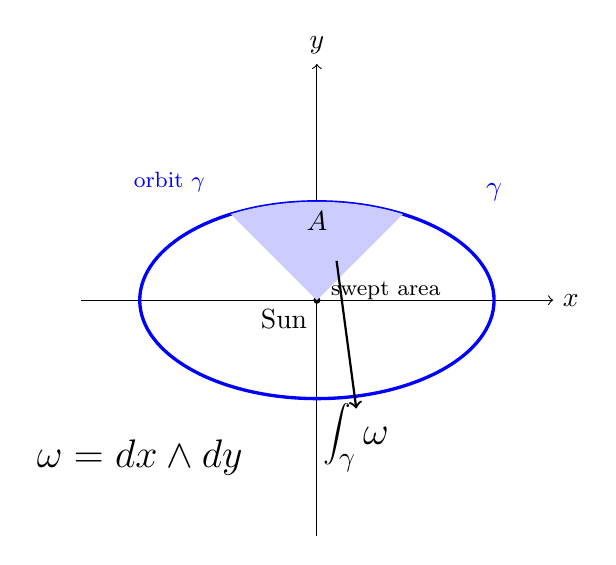
\begin{tikzpicture}[scale=2.5]
        % Coordinate axes
        \draw[->] (-1.2, 0) -- (1.2, 0) node[right] {$x$};
        \draw[->] (0, -1.2) -- (0, 1.2) node[above] {$y$};
    
        % Elliptical orbit (1-cycle)
        \draw[very thick, blue] (0.9, 0) arc[start angle=0, end angle=360, x radius=0.9, y radius=0.5];
        \node[blue] at (0.9, 0.55) {$\gamma$};
    
        % Focus (origin)
        \filldraw[black] (0,0) circle (0.015);
        \node[below left] at (0,0) {Sun};
    
        % Shaded swept area (2-form region)
        \begin{scope}
            \clip (0,0) -- (45:0.9) arc[start angle=45, end angle=135, x radius=0.9, y radius=0.5] -- cycle;
            \fill[blue!20] (0.9, 0) arc[start angle=0, end angle=360, x radius=0.9, y radius=0.5];
        \end{scope}
        \node at (0,0.4) {$A$};
    
        % Wedge notation for 2-form
        \node at (-0.9, -0.8) {\Large $\omega = dx \wedge dy$};
    
        % Integral expression
        \node at (0.2, -0.7) {\Large $\displaystyle \int_\gamma \omega$};
    
        % Arrow pointing from area to integral
        \draw[->, thick] (0.1, 0.2) -- (0.2, -0.55);
    
        % Labels
        \node at (0.35, 0.05) {\footnotesize swept area};
        \node[blue] at (-0.75, 0.6) {\footnotesize orbit $\gamma$};
    
    \end{tikzpicture}
    \caption{The pairing of a 1-cycle $\gamma$ (planetary orbit) with a closed 2-form $\omega$ gives the swept area: $\int_{\gamma} \omega$.}
    \label{fig:cohomological_orbit}
\end{figure}

\begin{tcolorbox}[colback=gray!5!white, colframe=gray!50!black, title={Summary}]
The motion of planets, the conservation of momentum, the optimization of trajectories—all emerge from the preservation of cohomological structure.

The laws of physics are not merely differential—they are topological.

\begin{quote}
\textbf{The universe evolves, yes—but in a way that respects its hidden invariants.}
\end{quote}
\end{tcolorbox}



\begin{tcolorbox}[colback=blue!5!white, colframe=blue!50!black, breakable, title={Historical Sidebar: If Kepler Had Known Cohomology}]

    Johannes Kepler spent years hunched over numbers, searching for harmony in the heavens.
    What he found—planets sweeping out equal areas in equal times—was, to him, a glimpse of divine order.
    Geometry whispered secrets. Ratios sang. The cosmos, he believed, was written in the language of music and math.
    
    But Kepler never knew just how deep the pattern went.
    
    Cohomology—the idea that hidden structures govern what can change and what must stay constant—would not be invented for another three centuries. It waited in the minds of Riemann, Poincaré, de Rham, and a host of others, still unborn.
    
    If Kepler had known, he would have realized:
    
    \begin{quote} He wasn’t just measuring areas.
    He was touching invariants—quantities so fundamental that no bending, twisting, or warping of the cosmos could erase them. \end{quote}
    
    His “equal areas” were not accidents of motion.
    They were shadows of a deeper conservation—\textbf{a preserved 2-form}, stitched into the fabric of space itself.
    
    The planets weren’t just obedient to God’s design;
    they were \emph{guardians of cohomological truth}.
    
    Had Kepler known, his hymns to cosmic harmony would have sounded even richer:
    
    \begin{quote} \textit{Not merely music of the spheres,
    but the conservation of sacred forms.} \end{quote}
    
    He wasn’t just watching planets dance.
    He was glimpsing the hidden algebra of the universe—
    written not in notes or chords, but in the eternal language of topology.
    
    And the areas he so carefully measured?
    
    They were the universe's way of whispering:
    
    \begin{quote} \textbf{Some patterns are too fundamental to break.} \end{quote}
    
\end{tcolorbox}


\subsection{Einstein’s Warning: Cohomology is Not Cosmology}

As we marvel at how cohomology explains so much—from conserved quantities to planetary orbits—it is tempting to fall into a trap Einstein himself warned against:

\begin{quote}
\textit{“As far as the laws of mathematics refer to reality, they are not certain;  and as far as they are certain, they do not refer to reality.”}  
\\[-0.5em]
\hfill --- Albert Einstein
\end{quote}

Einstein understood that mathematical structures—no matter how elegant—are tools for modeling experience, not the fabric of reality itself.  Spacetime, to him, was a \textit{framework}... not a thing. It is a mathematical convenience; not a metaphysical commitment.

\medskip

The same applies to cohomology.

Cohomology classifies structures. It reveals invariants. It describes what cannot be deformed away.  
But it does not dictate the material content of the universe. 

\begin{tcolorbox}[colback=red!5!white, colframe=red!50!black, title={Cautionary Note}]
\textbf{Cohomology is not cosmology.}  
It tells us what can be preserved within a given mathematical setting—but not what that setting ultimately represents.

Mathematical invariants are not physical laws. They are scaffolding for thought.
\end{tcolorbox}

\medskip


Einstein’s point was not to dismiss mathematical frameworks, but to \textbf{discipline our metaphors}.  
Use math to explore, to predict, to unify—but don’t mistake the map for the terrain.

Cohomology reveals structure. It tells us what forms can persist, what symmetries can be preserved, what shapes cannot be deformed away.  
But whether the universe obeys these constraints—or merely reflects them in some limited regime—is an open question. One that sits at the boundary of physics, philosophy, and metaphysics.


In that sense, cohomology is a kind of metaphysical litmus test: it shows us the deep architecture of possibility, whether or not the world chooses to inhabit it.

\begin{quote}
\textit{Mathematics is real. But reality is not necessarily mathematics.  In fact, mathematics may exist even beyond our reality. And, in some sense, that might make mathematics even more real than reality.}
\end{quote}



\begin{tcolorbox}[colback=blue!5!white, colframe=blue!75!black, breakable, title={Sidebar: Gödel, Einstein, and the Rotating Universe}, fonttitle=\bfseries]

    In 1949, Kurt Gödel—the greatest logician of his time and a close friend of Albert Einstein—published a startling solution to Einstein’s equations: a model of a \textbf{rotating universe} containing closed timelike curves. Gödel’s universe implied that, in principle, one could travel back in time simply by following a sufficiently large loop in spacetime.

    \medskip
    
    Einstein was both intrigued and philosophically uneasy with this discovery. While Einstein's own theories allowed for such solutions, he did not believe the real universe admitted them. Yet he deeply admired Gödel’s intellect. As Einstein himself quipped:
    \begin{quote}
    \textit{I go to my office just to have the privilege of going home with Kurt Gödel.}
    \end{quote}
    
    Freeman Dyson, then a young scholar at Princeton in 1948, recalled his first encounter with Gödel:

    \begin{quote}
    \small
    It was September 1948 and I had just become a young member of the Institute for Advanced Study. I was very surprised that one of the first people I met was Kurt Gödel himself, and I was even more surprised when he invited me to his house... We talked about physics. He knew physics very well... Einstein had proposed to him to analyze rotating universes and he had done it... Every time we saw each other, he would ask me: ‘Have they discovered it? Have they discovered whether the universe rotates?’ And I had to tell him no.
    \end{quote}
    
    Mathematically, Gödel’s rotating universe raised profound questions about the global structure of spacetime. The existence of closed timelike curves pointed to a \textbf{non-trivial topology}, hinting at deep connections with the cohomology of spacetime. In simple terms: if spacetime allows such loops, then its “global shape” cannot be trivial—there exist non-contractible loops that persist even in the presence of local flattening.

    \medskip
    
    Cohomology, which classifies global differential forms, provides a modern language for understanding such features. A rotating universe, with inherent “twist” in its causal structure, may correspond to a non-trivial cohomology class that obstructs trivializing the rotation globally. In this sense, Gödel’s universe wasn’t merely a curiosity—it was an early window into the topological and algebraic underpinnings of cosmology.

    \medskip
    
    And yet, for Gödel, it wasn’t just math or physics. It was a profound philosophical challenge to the nature of time itself.
    
\end{tcolorbox}
